%\chapter{Query Optimizer Integration}
\documentclass[10pt]{article} \begin{document} \label{discussion}

In the earlier sections, given a user query, the standard plan choice of the
PostgreSQL optimizer was used even with the modified operator implementations.
That is, while the execution engine was PCM-conscious, the presence of PCM was
completely \emph{opaque} to the optimizer.  However, given the read-write
asymmetry of PCM in terms of both latency and wear factor, it is possible that
alternative plans, capable of providing better performance profiles, may exist
in the plan search space. To discover such plans, the database query optimizer
needs to incorporate PCM awareness in both the operator cost models and the plan
enumeration algorithms.

Current query optimizers typically choose plans using a latency based costing
mechanism. We revise these models to account for the additional latency incurred
during writes. Additionally, we introduce a new metric of \emph{write cost} in
the operator cost model, representing the incurred writes for a plan, using the
estimators described in 
%Sections~\ref{sort}
to 
%\ref{gby}. 
We henceforth refer to the latency cost and the write cost of a plan as
\textbf{LC} and \textbf{WC}, respectively.

A new user-defined parameter, called the \emph{latency slack}, is incorporated
in the query optimizer.  This slack, denoted by $\lambda$, represents the
maximum relative slowdown, compared to the LC-optimal query plan, that is
acceptable to the user in lieu of getting better write performance.
Specifically, if the LC of the LC-optimal execution plan $P_o$ is $C_o$ and the
LC of an alternate plan $P_i$ is $C_i$, the user is willing to accept $P_i$ as
the final execution plan if $C_i \le (1+\lambda) C_o$. The $P_i$ with the least
WC satisfying this equation is considered the WC-optimal plan.

With the new metric in place, we need to revise the plan construction process
during the planning phase. This is because the native optimizer propagates just
the LC-optimal (and interesting order plans) through the internal nodes of the
dynamic programming lattice, which may lead to pruning of potential WC-optimal
plans. On the other hand, propagating the \emph{entire} list of sub-plans at
each internal node can end up in an exponential blowup of the search space. One
immediate pruning technique is to to discard each plan that is dominated by some
other plans in both LC and WC metrics.

To examine the nature of WC-optimal plans, we conducted an exhaustive
enumeration for a limited subset of plans in the TPC-H benchmark. In all the
experiments, we observed that the WC-optimal plan invariably had the same join
order as the LC-optimal plan. The intuitive explanation of this can be that the
join order chosen in the LC-optimal plan was picked up because it involved
lesser data processing. Using a different join order then would translate to
more data and consequently more writes.


Keeping this observation in mind, the problem of finding the WC-optimal plan can
be mapped to the well known variation of the knapsack problem (KP) called the
\emph{Linear Multiple Choice Knapsack Problem (LMCKP)}. Each item in LMCKP has a
weight and a profit associated with it like KP, and these items are divided into
disjoint sets. The objective is to pick up one item from each set in such a
manner that the total weight of the items is within the maximum weight allowed
in the knapsack, while maximising the total profit obtained. Formally stated,
the LMCKP problem is as follows:

We are given multiple sets $S_1, S_2,..., S_k$ of items to be packed in a
knapsack of capacity $c$. For each item $j \in S_i$ , there is an associated
profit $p_{ij}$ and a weight $w_{ij}$. The objective is to choose one item from
each class so as to maximize the profit sum while having the weight sum to be
within c. Formally, the Linear Multiple Choice Knapsack Problem (LMCKP) may thus
be formulated as:

maximize $z = \sum\limits_{i=1}^{k} \sum\limits_{j \in S_i}p_{ij} x_{ij}$

subject to $\sum\limits_{i=1}^{k} \sum\limits_{j \in S_i}w_{ij}  x_{ij} \le c$,

$\sum\limits_{j \in S_i}$    $ x_{ij} = 1, i = 1,...,k$

$0 \le x_{ij} \le 1$, $i = 1,...,k, j \in S_i$

All coefficients $p_{ij}, w_{ij}$, and $c$ are positive integers, and the
classes $S_1$,...$S_k$ are mutually disjoint, class $S_i$ having size $s_i$. The
total number of items is $n = \sum\limits_{i=1}^{k} n_i$


In our case, the weight of each item can be equated to the response time
associated with each operator execution algorithm. The target of maximising the
profit can similarly be mapped to minimising the writes, by changing their sign
to negative and then adding a common large positive constant to each of them. We
use MWC to refer to this modified WC.

We use a greedy algorithm to solve the LMCKP \cite{lmckp}.  We find the convex
hull (LP-dominating set) of points $L_i$ in the 2-D space ordered by LC on the
x-axis and the MWC on the y-axis, for each class $S_i$. We then begin by
choosing the least LC item in each class (i.e. we set $x_{i1} = 1, x_{ij} = 0$
for $j=2,...,|L_i|, i = 1,...,k$). The weight and profit sums for the chosen
items can then be defined as 

$W = \sum\limits_{i=1}^{k} w_{i1}$ and 

$P = \sum\limits_{i=1}^{k} p_{i1}$, 

respectively. For all items $j \neq 1$, we define the slope $\lambda_{ij}$ as 

$\lambda_{ij} = \dfrac {p_{ij} - p_{i,j-1} }{w_{ij} - w_{i,j-1}}$

This slope is a measure of the profit to weight ratio obtained by choosing item
$j$ instead of item $j-1$ in class $R_i$. Using the greedy principle, order the
slopes $\lambda_{ij}$ in non-increasing order.

Let $i,j$ be the indices corresponding to the next slope $\lambda_{ij}$ in
$\{\lambda_{ij}\}$ . If $W + w_{ij} > c$, goto Step 3. Otherwise set $x_{ij} =
1, x_{i, j-1} = 0$ and update the sume $W = W + w_{ij} - w_{i,j-1}, P = P +
p_{ij} - p_{i,j-1}, $. Repeat Step 2

If $W=c$ we have an integer solution and the optimal objective value to LMCKP is
$z^* = P$. Otherwise let $\lambda_{ij}$ be the next slope in the list. We have
two fractional variables $x_{ij} = \dfrac {c-W}{w_{ij} - w_{i,j-1}}$ and
$x_{i,j-1} = 1 - x_{ij}$ respectively, which both belong to the same class. The
optimal objective value is 

$z^* = P + (c-W)\lambda_{ij}$

In this scenario, we perform a partial execution of an operator with one
algorithm and the remaining execution with the second algorithm, the algorithms
corresponding to the $(j-1)$th and $j$th operator algorithms at the $i$th node.
In case of join nodes for example, the inner relation can be divided into two
parts in the ratio of the weights obtained from the greedy algorithm. One part
can be joined to the entire outer relation with one algorithm and the other part
with the second algorithm.

With the above background in place, we describe our final algorithm which uses
two-passes to come up with the WC-optimal plan:

\subsection*{First Pass} In the first pass, we keep track of the LC-optimal and
an additional least WC plan (similar in the way of tracking interesting order
plans) using the usual dynamic programming procedure. If they both are the same,
we skip the second pass and output that plan as the solution.

\subsection*{Second Pass} In this pass, we start with the least latency
algorithm at each node. Afterwards, we follow the greedy procedure for LMCKP
problem and come up with the WC-optimal plan using the cost bound obtained
through the LC-optimal plan found in the first pass. 

In light of these modifications, let us revisit Query Q13, for which the default
plan was shown in Figure~\ref{fig:plan_trees}(a). With just the revised latency
costs (i.e. $\lambda$ = 0), the optimizer identified a new execution plan
wherein the merge left join between the \textit{customer} and \textit{orders}
tables is replaced by a hash left join. The relative performance of these two
alternatives with regard to PCM Writes and Cycles are shown in
Figure~\ref{fig:perf_comp}(a). We observe here that there is a \emph{huge
difference} in both the query response times as well as writes overheads for
both the plans.  Specifically, the alternative plan reduces the writes by well
over an order of magnitude!  As we gradually increased the latency slack value,
we initially didn't notice any change in plans. However, when the slack was made
as large as 5, the hash left join gave way to nested loop left join, clearly
indicating that it gives write savings at a steep increase in latency cost.


%\begin{figure}[htbp] \centering
%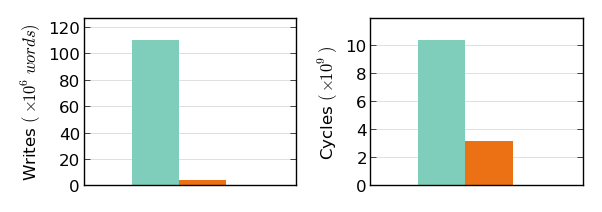
\includegraphics[height=29mm]{q13_alternate_plan.png} \caption{Performance of
%Alternative Plans} \label{fig:perf_comp} \end{figure}	
%
%
\begin{table}[!h] \centering \caption{Overall performance comparison}
\label{fig:perf_comp} \begin{tabular}{p{2.8cm}p{2.5cm}p{2.5cm}p{2.5cm}p{2.5cm}}
\toprule
\textbf{Metric} & \textbf{Optimizer (PCM-O) Executor (PCM-O) } &
\textbf{Optimizer (PCM-O) Executor (PCM-C)} & \textbf{Optimizer (PCM-C) Executor
(PCM-C)} & \textbf{Optimizer (PCM-C) Executor (PCM-O)}\\ \midrule                                                                                                

\textbf{Writes(words)} &  $233.6 \times 10^6$ & $110.6 \times 10^6$ & $4.66
\times 10^6$ & $12.8 \times 10^6$\\ \textbf{Cycles} &  $13.1 \times 10^9$ &
$10.4 \times 10^9$ & $3.2 \times 10^9$ & $4.5 \times 10^9$\\ \bottomrule
\end{tabular}
\end{table}



To put matters into perspective, Figure~\ref{fig:perf_comp}(b) summarizes the
relative performance benefits obtained as the database layers are gradually made
PCM-conscious (in the figure, the labels Opt and Exec refer to Optimizer and
Executor, respectively, while PCM-O and PCM-C refer to PCM-Oblivious and
PCM-Conscious, respectively). For the sake of completeness, we have also added
results for the case when the Optimizer is PCM-C but the Executor is PCM-O (last
column). The results clearly indicate that future query optimizers for PCM-based
architectures need to incorporate PCM-Consciousness at \emph{both} the Optimizer
and the Executor level in order to get the best performance while executing a
given query.




%\begin{figure}[h] %\centering \subfloat[Database layers]{
%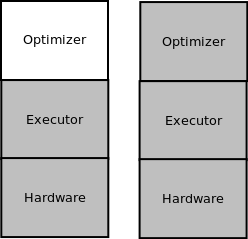
\includegraphics[width=4cm]{db_levels.png} } \subfloat[Q13 alternate plan]{
%\begin{tikzpicture}[scale=., transform shape]
%
%\tikzstyle{every node} = [rectangle, fill=gray!5]
%
%\node (d) at (0,3) {Index Scan / Filter}; \node (c) at (0,1.5) {CUSTOMER};
%
%\node (s) at (3,3) {Hash}; \node (p) at (3,2.25) {Seq. Scan / Filter}; \node
%(a) at (3,1.5) {ORDERS};
%
%\node (e) at (1.5,4) {Hash Left Join}; \node (f) at (1.5,5)  {Group Aggregate};
%\node (g) at (1.5,6)  {Hash Aggregate}; \node (h) at (1.5,7)  {Sort};
%
%
%\draw[-] (c) -- (d); \draw[-] (a) -- (p); \draw[-] (d) -- (e); \draw[-] (p) --
%(s); \draw[-] (s) -- (e); \draw[-] (e) -- (f);
%
%\draw[-] (f) -- (g); \draw[-] (g) -- (h);
%
%\end{tikzpicture} } %\centering                                                                                             
%
%\caption{Alternative Execution Plans for Query Q13} \label{fig:layers}
%	
%\end{figure}

\end{document}
